\documentclass[border=3pt,tikz]{standalone}
% Shared look for every TikZ figure in these notes.
% Included by each standalone figure file; also keeps the figures consistent
% with the colours used in the PDF and on the website.

\usepackage{tikz}
\usepackage{pgfplots}
\pgfplotsset{compat=1.18}
\usetikzlibrary{arrows.meta, decorations.markings, decorations.pathmorphing,
                patterns, calc, positioning}
\usepackage{amsmath}

% Series colours are the three validated categorical slots also used by the
% interactive widgets, so a path drawn in the printed notes and the same path on
% the website are the same colour. They clear the colour-vision-deficiency and
% contrast checks as a set; every path is direct-labelled as well, so colour is
% never the only thing carrying identity.
\definecolor{duPurple}{HTML}{68246D}
\definecolor{duBlue}{HTML}{2A78D6}
\definecolor{duRed}{HTML}{EB6834}
\definecolor{duGreen}{HTML}{1BAF7A}
\definecolor{duGrey}{HTML}{6B6B6B}

\tikzset{
  axisline/.style   = {-{Stealth[length=3mm]}, line width=0.7pt, black},
  path1/.style      = {duBlue,   line width=1.1pt},
  path2/.style      = {duRed,    line width=1.1pt},
  path3/.style      = {duGreen,  line width=1.1pt},
  statedot/.style   = {circle, fill=black, inner sep=1.4pt},
  arrowhead/.style  = {decoration={markings,
                        mark=at position #1 with {\arrow{Stealth[length=2.6mm]}}},
                       postaction={decorate}},
  lbl/.style        = {font=\small},
  slbl/.style       = {font=\footnotesize, duGrey},
  workfill/.style   = {duPurple, opacity=0.16},
}

\usetikzlibrary{shapes.geometric}
% Corollary 5: a heat engine exchanging heat with several reservoirs
\begin{document}
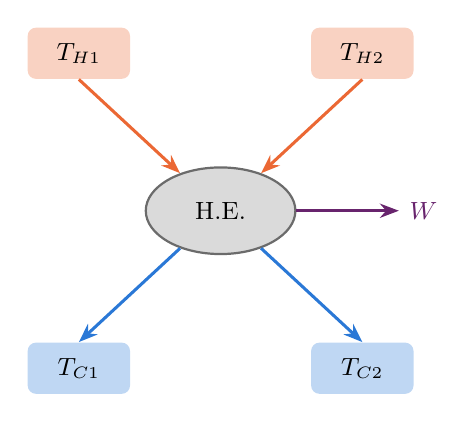
\begin{tikzpicture}[x=1cm,y=1cm,
    resv/.style={draw=none, rounded corners=3pt, minimum width=1.3cm, minimum height=0.65cm, font=\small},
    eng/.style={ellipse, draw=duGrey, fill=duGrey!25, line width=0.8pt, minimum width=1.9cm, minimum height=1.1cm, font=\small},
    flow/.style={-{Stealth[length=2.4mm]}, line width=1.1pt}]
  \node[eng] (E) at (0,0) {H.E.};
  \node[resv, fill=duRed!30] (H1) at (-1.8,2) {$T_{H1}$};
  \node[resv, fill=duRed!30] (H2) at (1.8,2) {$T_{H2}$};
  \node[resv, fill=duBlue!30] (C1) at (-1.8,-2) {$T_{C1}$};
  \node[resv, fill=duBlue!30] (C2) at (1.8,-2) {$T_{C2}$};
  \draw[flow, duRed] (H1.south) -- (E);
  \draw[flow, duRed] (H2.south) -- (E);
  \draw[flow, duBlue] (E) -- (C1.north);
  \draw[flow, duBlue] (E) -- (C2.north);
  \draw[flow, duPurple] (E.east) -- ++(1.3,0) node[right, lbl] {$W$};
\end{tikzpicture}
\end{document}
